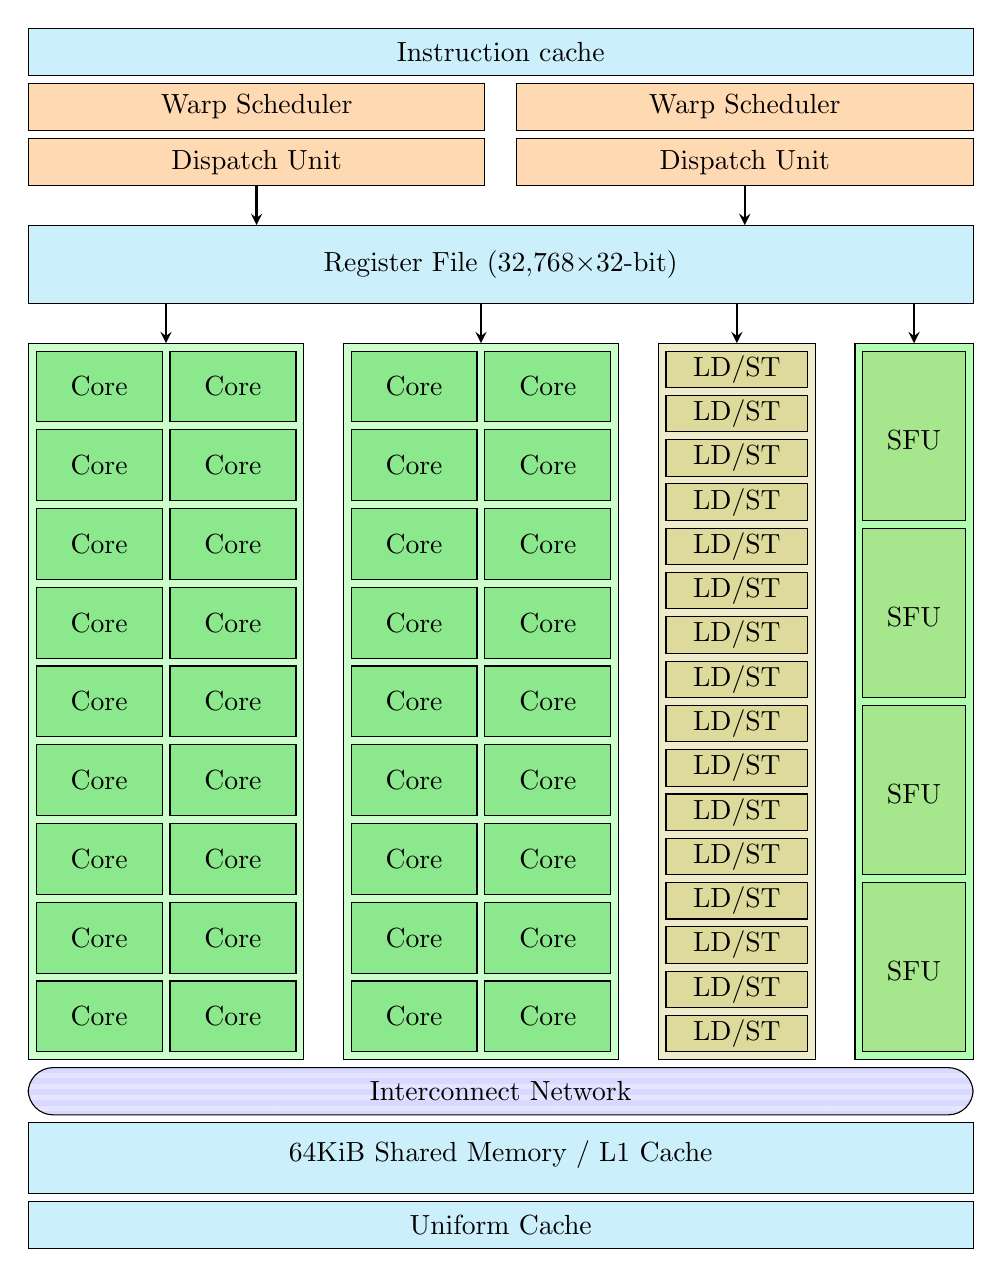
\begin{tikzpicture}[>=stealth]
\usetikzlibrary{patterns}

\draw[fill=cyan!20] (0,0) rectangle ++(12,-0.60);
\draw node at (6,-0.30) {Instruction cache};

\draw[fill=orange!30] (0,-0.7) rectangle ++(5.8,-0.6);
\draw node at (2.9, -1) {Warp Scheduler};

\draw[fill=orange!30] (6.2,-0.7) rectangle ++(5.8,-0.6);
\draw node at (6.2 + 2.9, -1) {Warp Scheduler};

\draw[fill=orange!30] (0,-1.4) rectangle ++(5.8,-0.6);
\draw node at (2.9, -1.7) {Dispatch Unit};

\draw[fill=orange!30] (6.2,-1.4) rectangle ++(5.8,-0.6);
\draw node at (6.2 + 2.9, -1.7) {Dispatch Unit};

\draw[->, thick] (2.9,-2) -- (2.9,-2.5);
\draw[->, thick] (6.2+2.9,-2) -- (6.2+2.9,-2.5);

\draw[fill=cyan!20] (0,-2.5) rectangle ++(12,-1);
\draw node at (6, -2.5-0.5) {Register File (32,768$\times$32-bit)};

\draw[->,thick] (1.75,-3.5) -- ++(0,-0.5);
\draw[->,thick] (5.75,-3.5) -- ++(0,-0.5);

\foreach \x in {0,4}
{
  \draw[fill=green!20] (\x, -4) rectangle (\x+3.5, -13.1);
  \foreach \j in {0,...,8}
  {
    \foreach \k in {0 ,1.7}
    {
      \draw[fill=green!80!black!45] (\x+0.1+\k, -4 - \j*1 -0.1) rectangle ++(1.6,-0.9);
      \draw node at (\x+0.1+\k+0.8, -4 - \j*1 -0.1-0.45) {Core};
    }
  }
}

\draw[->,thick] (9,-3.5) -- ++(0,-0.5);
\draw [fill=olive!15] (8.0,-4) rectangle (10,-13.1);
\foreach \x in {0,...,15}
{
  \draw [fill=olive!30] (8.1, -4.1 - 9.0/16 * \x) rectangle ++(1.8, -9.0/16.0+0.1);
  \draw node at (8.1 + 0.9, -4.1 - 9.0/16 * \x  - 9.0/16.0/2+0.1/2) {LD/ST};
}

\draw[fill=green!30] (10.5, -4) rectangle (12,-13.1);
\draw[->,thick] (10.5 + 0.75,-3.5) -- ++(0,-0.5);
\foreach \x in {0,...,3}
{
  \draw[fill=green!60!brown!50] (10.6, -4.1 - 9.0/4*\x) rectangle ++(1.3, -9.0/4+0.1);
  \draw node at  (10.6 + 1.3/2, -4.1 - 9.0/4*\x - 9.0/4/2) {SFU};
}

\draw[pattern=horizontal lines light blue,rounded corners=9pt] (0,-13.2) rectangle ++(12,-0.60);
\draw node at (6,-13.50) {Interconnect Network};

\draw[fill=cyan!20] (0,-13.9) rectangle ++(12,-0.90);
\draw node at (6,-14.30) {64KiB Shared Memory / L1 Cache};

\draw[fill=cyan!20] (0,-14.9) rectangle ++(12,-0.60);
\draw node at (6,-15.20) {Uniform Cache};

\end{tikzpicture}